\documentclass{article} % For LaTeX2e
\usepackage{nips14submit_e,times}
\usepackage{amsmath}
\usepackage{amsthm}
\usepackage{amssymb}
\usepackage{mathtools}
\usepackage{hyperref}
\usepackage{url}
\usepackage{algorithm}
\usepackage[noend]{algpseudocode}
%\documentstyle[nips14submit_09,times,art10]{article} % For LaTeX 2.09

\usepackage{graphicx}
\usepackage{caption}
\usepackage{subcaption}

\def\eQb#1\eQe{\begin{eqnarray*}#1\end{eqnarray*}}
\def\eQnb#1\eQne{\begin{eqnarray}#1\end{eqnarray}}
\providecommand{\e}[1]{\ensuremath{\times 10^{#1}}}
\providecommand{\pb}[0]{\pagebreak}
\DeclarePairedDelimiter\ceil{\lceil}{\rceil}
\DeclarePairedDelimiter\floor{\lfloor}{\rfloor}

\newcommand{\E}{\mathrm{E}}
\newcommand{\Var}{\mathrm{Var}}
\newcommand{\Cov}{\mathrm{Cov}}

\def\Qb#1\Qe{\begin{question}#1\end{question}}
\def\Sb#1\Se{\begin{solution}#1\end{solution}}

\newenvironment{claim}[1]{\par\noindent\underline{Claim:}\space#1}{}
\newtheoremstyle{quest}{\topsep}{\topsep}{}{}{\bfseries}{}{ }{\thmname{#1}\thmnote{ #3}.}
\theoremstyle{quest}
\newtheorem*{definition}{Definition}
\newtheorem*{theorem}{Theorem}
\newtheorem*{lemma}{Lemma}
\newtheorem*{question}{Question}
\newtheorem*{preposition}{Preposition}
\newtheorem*{exercise}{Exercise}
\newtheorem*{challengeproblem}{Challenge Problem}
\newtheorem*{solution}{Solution}
\newtheorem*{remark}{Remark}
\usepackage{verbatimbox}
\usepackage{listings}
\title{Probabilistic Method: \\
Problem Set IV}


\author{
Youngduck Choi \\
CIMS \\
New York University\\
\texttt{yc1104@nyu.edu} \\
}


% The \author macro works with any number of authors. There are two commands
% used to separate the names and addresses of multiple authors: \And and \AND.
%
% Using \And between authors leaves it to \LaTeX{} to determine where to break
% the lines. Using \AND forces a linebreak at that point. So, if \LaTeX{}
% puts 3 of 4 authors names on the first line, and the last on the second
% line, try using \AND instead of \And before the third author name.

\newcommand{\fix}{\marginpar{FIX}}
\newcommand{\new}{\marginpar{NEW}}

\nipsfinalcopy % Uncomment for camera-ready version

\begin{document}


\maketitle

\begin{abstract}
This work contains solutions to the problem set IV
of Probabilistic Method 2016 at Courant Institute of Mathematical Sciences.
\end{abstract}

\bigskip

\begin{question}[1]
\hfill
\begin{figure}[h!]
  \centering
    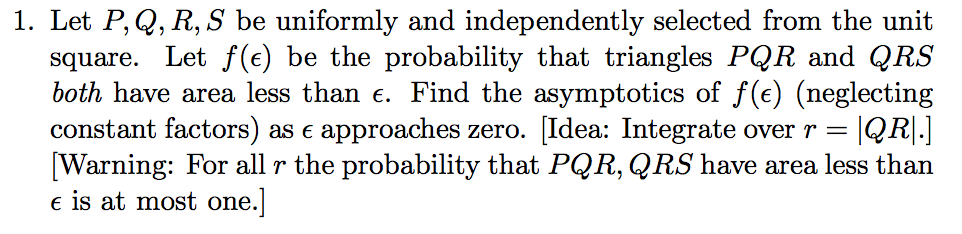
\includegraphics[width=1\textwidth]{PM-4-1.png}
\end{figure}
\end{question}
\begin{solution}
From the analysis of the combinatorial geometry section $3.3$, it follows that
\eQb
Pr(b \leq |QR| \leq b + db) \leq 2\pi b db,
\eQe
where $b$ denotes the distance between $P$ and $R$. Given the distance $b$, we must
have $h < \dfrac{2\epsilon}{b}$ to ensure that the area is less than $\epsilon$. 
An upper bound to the area of such region is $4\dfrac{2\epsilon}{b}\sqrt{2} = 
\dfrac{4\sqrt{2}\epsilon}{b}$, which can be seen from using the $\sqrt{2}$
middle strip. Now, the probability that $S$ lies in such region is
thus, $\max(\dfrac{4\sqrt{2}\epsilon}{b},1)$. As we need to compute the probability
of both $PQR$ and $QRS$ having an area smaller than $\epsilon$, 
the total probability is bounded by
\eQb
f(\epsilon) &\leq& \int_{b=0}^{\sqrt{2}} 2\pi b [\max(\dfrac{4\sqrt{2}\epsilon}{b}, 1)]^2 db.
\eQe
When $b \leq \dfrac{\epsilon}{4\sqrt{2}}$, we have the max term is simply $1$. Hence, using
the additivity of integral, we have
\eQb
f(\epsilon) &\leq& \int_{b=0}^{4\sqrt{2}\epsilon} 2
\pi b [\max(\dfrac{4\sqrt{2}\epsilon}{b}, 1)]^2 db.
+ c \int_{b= 4\sqrt{2} \epsilon}^{1} \dfrac{\epsilon^2}{b} db, 
\eQe
where $c$ is the constant associated from the original integral. Now, observe that the 
first integral is $O(\epsilon^2)$ and the second integral is $O(\epsilon^2 \ln(\epsilon^{-1}))$.
Therefore, we have shown that $f(\epsilon) = O(\epsilon^2 \ln(\epsilon))$.
\hfill $\qed$
\end{solution}

\newpage

\begin{question}[2]
\hfill
\begin{figure}[h!]
  \centering
    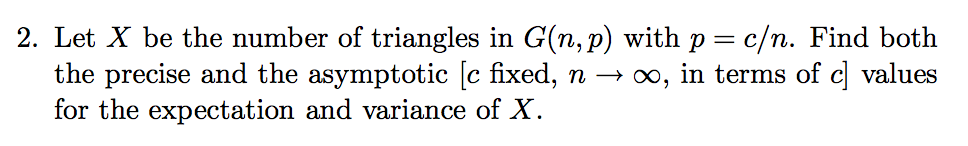
\includegraphics[width=1\textwidth]{PM-4-2.png}
\end{figure}
\end{question}
\begin{solution} For every 3-set $S$ of vertices in $G(n,p)$,
let $A_S$ be the event that $S$ is a triangle. In particular, we have $X = \sum_{S} X_S$.
By Linearity of Expectation, obtain
\eQb
E[X] &=& \sum_{S} E[X_S] = {n \choose 3} p^3 = {n \choose 3} (\dfrac{c}{n})^3 \sim \dfrac{1}{6}c^3.   
\eQe
Now, by definition of variance, we have
\eQb
Var[X] &=& \sum_{S} Var[X_S] + \sum_{S \neq T} Cov[X_S, X_T].
\eQe
Using the variance formula for discrete random variable, we 
have that
\eQb
\sum_{S} Var[X_S] &=& {n \choose 3} p^3(1-p^3). 
\eQe
As $p = o(1)$, we have that $(1-p^3) = o(1)$. Therefore, we can further deduce
\eQb
Var[X_S] &=& p^3 (1-p^3) \sim p^3 \> \text{ and } \> Var[X_S] \sim E[X_S] \sim \dfrac{1}{6}c^3. 
\eQe 
Now, observe that covariance is $0$ for $S,T$ pair, where $|S \cap T| \neq 2$. Now, for $S,T$ pair,
where $|S \cap T| = 2$, we have, by definition of covariance, 
\eQb
Cov(X_S, X_T) &=& E[X_S X_T] - E[X_S]E[X_T] = p^5 - p^6.
\eQe
Since there are ${n \choose 3} 3 (n-3)$ choices (fix the first triangle, pick the one that will not
be shared, and choose the remaining one from the rest of the graph), we finally have
\eQb
\sum_{S \neq T} Cov(X_S, X_T) &=& {n \choose 3} 3 (n-3) (p^5 - p^6) = o(1).
\eQe
Therefore, we can conclude that $Var[X] \sim \dfrac{c^3}{6}$ as well. Reminds me of Poisson, 
but not gonna think too hard about it for now. \hfill $\qed$
\end{solution}

\newpage

\begin{question}[3]
\hfill
\begin{figure}[h!]
  \centering
    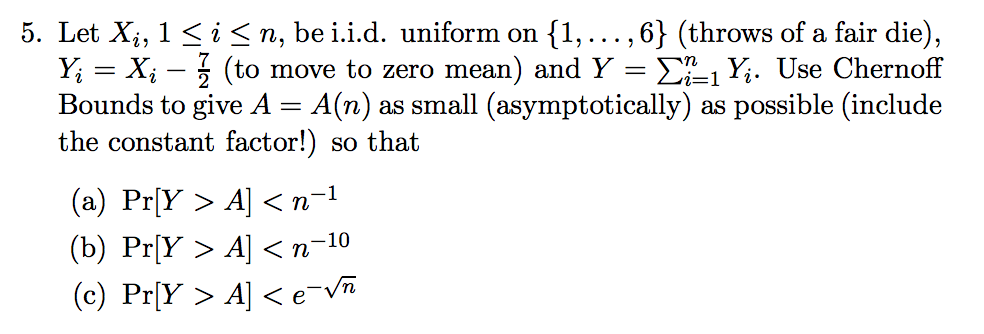
\includegraphics[width=1\textwidth]{PM-4-3.png}
\end{figure}
\end{question}
\begin{solution}
With simple computation, we can see that
\eQb
\sigma_i^2 = \dfrac{35}{12} \> \text{ and } \> \sigma_2 = \dfrac{35}{12}.
\eQe
As $Y_i$ are uniformly bounded, by the use of Chernoff bound, it follows that
\eQb
P(Y > a\sigma ) < e^{-\frac{a^2}{2}(1+o(1))}.
\eQe
Therefore, we must have $\frac{a^2}{2} = \ln(n), 10\ln(n) , \sqrt{n}$. Solving these respectively,
we obtain that $a = (2\ln(n))^{\frac{1}{2}}, (20\ln(n))^{\frac{1}{2}}, 2^{\frac{1}{2}} n^{\frac{1}{4}}$.
\hfill $\qed$ 
\end{solution}

\end{document}

